% !TEX root = ../projektdokumentation.tex

\section{Projektdurchführung}\label{projektdurchfuehrung}
\section{Projektdurchführung}\label{projektdurchfuehrung}

\subsection{Vorgehensmodell}\label{vorgehensmodell}

Für die Projektdurchführung wurde das agile Vorgehensmodell \gls{Scrum} gewählt. Scrum ist ein weit verbreitetes Framework für die agile Softwareentwicklung, das iterative und inkrementelle Prozesse unterstützt. Es besteht aus festen Rollen, Ereignissen und Artefakten, die bei der iterativen Softwareentwicklung unterstützen. Aufgrund der kurzen Projektdauer und der unregelmäßigen Verfügbarkeit der Teammitglieder wurde eine angepasste Version von Scrum verwendet, die die Flexibilität und Anpassungsfähigkeit des Frameworks beibehält, aber an die spezifischen Anforderungen des Projekts angepasst ist.

Der Methodologie von Scrum folgend wurde das Projekt in drei Sprints unterteilt, wobei die Sprints abweichend von der Regel zwischen drei und sechs Wochen dauerten. Diese zusätzliche Flexibilität ermöglichte es dem Team, sich besser an die Anforderungen und den Fortschritt des Projekts anzupassen. Jeder Sprint wurde mit einem Sprint-Planungsmeeting gestartet, in dem die Ziele und Aufgaben für den Sprint festgelegt wurden. Während des Sprints fanden regelmäßige Weekly-Meetings\footnote{Scrum sieht zwar Daily-Meetings vor, doch aufgrund der unregelmäßigen Verfügbarkeit der Teammitglieder wurden wöchentliche Meetings abgehalten.} statt, um den Fortschritt zu überprüfen und Hindernisse zu beseitigen. Am Ende jedes Sprints wurde ein Sprint Review Meeting abgehalten, um die erreichten Ziele zu präsentieren und Feedback zu sammeln. In Abbildung \ref{fig:gantt-diagramm} auf Seite \pageref{fig:gantt-diagramm} sind die drei Sprints und ihre Phasen dargestellt.

Normalerweise sind Rollen und Verantwortlichkeiten in Scrum klar definiert. In diesem Projekt wurden die Rollen jedoch flexibel gehandhabt, da die Teammitglieder unterschiedliche Fähigkeiten und Verfügbarkeiten hatten. Die Teammitglieder übernahmen je nach Bedarf verschiedene Rollen, um sicherzustellen, dass die Anforderungen des Projekts erfüllt wurden. Die wichtigsten Rollen waren:

\begin{itemize}
    \item \textbf{Projektleitung}: Scrum sieht die Rolle des Projektleiters nicht vor, dennoch erschien es dem ganzen Team wichtig, eine Person zu haben, die verantwortlich für die Planung, Koordination und Überwachung des Projekts zeichnete – Christopher Spencer. Er stellte sicher, dass die Ziele erreicht und Hindernisse beseitigt wurden.
    \item \textbf{Backend}: Die Implementierung der Backend-Funktionalität und die Integration von Datenbanken und APIs programmierten in erster Linie Christopher Spencer und Justus Sieweke.
    \item \textbf{Frontend}: Die Implementierung der Benutzeroberfläche und die Interaktion mit dem Backend erledigte Jan Mahnken.
    \item \textbf{Plugins}: Die Implementierung von Plugins des Bot-Frameworks wurde in Arbeitsteilung von Philipp Batelka, Jahn Mahnken, Daniel Quellenberg, Fabian Reichwald, Justus Sieweke und Christopher Spencer erledigt. Die Entwickler arbeiteten eng zusammen, um die Anforderungen umzusetzen und den Code zu überprüfen.
    \item \textbf{Dokumentation und Marketing}: Verantwortlich für die Erstellung und Pflege der Projektdokumentation, der Projektpräsentation und des Marketingpitches waren Philipp Batelka, Daniel Quellenberg und Fabian Reichwald. Sie sorgten dafür, dass alle wichtigen Informationen und Entscheidungen dokumentiert wurden.
\end{itemize}

Ein großer Vorteil der verteilten Verantwortlichkeiten lag darin, dass die unterschiedlichen Fähigkeiten und Erfahrungen der Teammitglieder optimal genutzt werden konnten. Dies ermöglichte es jedem Einzelnen das Team genau in den Aufgaben zu unterstützen, für die sie am besten geeignet waren. 

Als Projektmanagement-Tool wurde \gls{Jira} eingesetzt. Die Planung, Durchführung und Überwachung des Projekts wurde dadurch klar und transparent. In Jira wurden die Anforderungen, Aufgaben, Sprints und Fortschritte des Projekts verwaltet. Dies ermöglichte es dem Team, den Überblick über den Projektfortschritt zu behalten, Hindernisse zu identifizieren und die Zusammenarbeit zu verbessern. Für die Versionsverwaltung waren \gls{Git} in Verbindung mit \gls{GitHub} die Werkzeuge der Wahl. Git ermöglichte es dem Team, den Code effizient zu verwalten, Änderungen nachzuverfolgen und Versionskonflikte zu lösen. GitHub wurde als zentrale Plattform für die Zusammenarbeit genutzt, um den Code zu teilen, \gls{Pull-Requests} zu überprüfen und Feedback zu geben. Die Entscheidung viele Repositories zu erstellen, ermöglichte es, den Code für verschiedene Komponenten und Module getrennt zu halten und die Verantwortlichkeiten klar zu trennen.

% Hier Gantt-Diagramm einfügen
\begin{sidewaysfigure}
\begin{ganttchart}[
  % ,canvas/.append style={draw=none}
  ,vgrid
  ,hgrid
  ,x unit=.85cm
  ,y unit chart=.85cm
  % ,title/.style={draw=none, fill=none}
  ,title height=1,
  ,title label font=\bfseries\footnotesize
  ,bar/.style={draw=none}
  ,bar label font=\small
  ,bar/.append style={fill=gantt-sprint}
  ,bar height=0.6
  ,bar label node/.append style={align=left}
  ,milestone/.style={draw=none}
  ,milestone/.append style={fill=gantt-milestone}
  ,milestone height=0.6
  ,milestone label font=\small
  ,group/.style={draw=none}
  ,group label font=\bfseries
  ,group/.append style={fill=gantt-iteration}
  ,group height=0.6
  ,group peaks width=0
  ,group left shift=0
  ,group right shift=0
  ,group label node/.append style={align=left}
  ,link/.append style={-latex}
]{1}{16}

  \gantttitle{Februar 2024}{3}
  \gantttitle{März 2024}{4} 
  \gantttitle{April 2024}{4}
  \gantttitle{Mai 2024}{5} \\
  \gantttitle{Sprint 1}{7}
  \gantttitle{Sprint 2}{6}
  \gantttitle{Sprint 3}{3}\\
  \gantttitle{\footnotesize KW 7}{1}
  \gantttitle{KW 8}{1}
  \gantttitle{KW 9}{1}
  \gantttitle{KW 10}{1}
  \gantttitle{KW 11}{1}
  \gantttitle{KW 12}{1}
  \gantttitle{KW 13}{1}
  \gantttitle{KW 14}{1}
  \gantttitle{KW 15}{1}
  \gantttitle{KW 16}{1}
  \gantttitle{KW 17}{1}
  \gantttitle{KW 18}{1}
  \gantttitle{KW 19}{1}
  \gantttitle{KW 20}{1}
  \gantttitle{KW 21}{1} 
  \gantttitle{KW 22}{1} \\
  
  % Sprint 1
  \ganttgroup{Sprint 1}{1}{7} \\
  \ganttbar[name=elem0]{Anforderungsanalyse}{1}{1} \\
  \ganttbar[name=elem1]{Design}{2}{7} \\
  \ganttbar[name=elem2]{Implementierung}{4}{7} \\
  \ganttmilestone[name=Sprint1Ende]{Sprint 1 Ende / Retro / Planung}{7} \\[grid]

  % Sprint 2
  \ganttgroup{Sprint 2}{8}{13} \\
  \ganttbar[name=elem3]{Implementierung}{8}{10} \\
  \ganttbar[name=elem4]{Testen}{11}{12} \\
  \ganttbar[name=elem5]{Integration}{13}{13} \\
  \ganttmilestone[name=Sprint2Ende]{Sprint 2 Ende / Retro / Planung}{13} \\[grid]

  % Sprint 3
  \ganttgroup{Sprint 3}{14}{16} \\
  \ganttbar[name=elem6]{Fehlerbehebung}{14}{15} \\
  \ganttbar[name=elem7]{Feinschliff und Dokumentation}{16}{16} \\
  \ganttmilestone[name=Sprint3Ende]{Sprint 3 Ende / Retro / Planung}{16} \\

  % Relations 
  % \ganttlink{elem0}{elem1}
  % \ganttlink{elem1}{elem2} 
  % \ganttlink{elem2}{Sprint1Ende}
  % \ganttlink{elem3}{elem4} 
  % \ganttlink{elem4}{elem5} 
  % \ganttlink{elem5}{Sprint2Ende} 
  % \ganttlink{elem6}{elem7} 
  % \ganttlink{elem7}{Sprint3Ende}
  
\end{ganttchart}
\caption{Gantt-Diagramm der Projektphasen}\label{fig:gantt-diagramm}
\end{sidewaysfigure}
Für die Projektdurchführung wurde das agile Vorgehensmodell \gls{Scrum} gewählt. Scrum ist ein weit verbreitetes Framework für die agile Softwareentwicklung, das iterative und inkrementelle Prozesse unterstützt. Es besteht aus festen Rollen, Ereignissen und Artefakten, die bei der iterativen Softwareentwicklung unterstützen. Aufgrund der kurzen Projektdauer und der unregelmäßigen Verfügbarkeit der Teammitglieder wurde eine angepasste Version von Scrum verwendet, die die Flexibilität und Anpassungsfähigkeit des Frameworks beibehält, aber an die spezifischen Anforderungen des Projekts angepasst ist.

Der Methodologie von Scrum folgend wurde das Projekt in drei Sprints unterteilt, wobei die Sprints abweichend von der Regel zwischen drei und sechs Wochen dauerten. Diese zusätzliche Flexibilität ermöglichte es dem Team, sich besser an die Anforderungen und den Fortschritt des Projekts anzupassen. Jeder Sprint wurde mit einem Sprint-Planungsmeeting gestartet, in dem die Ziele und Aufgaben für den Sprint festgelegt wurden. Während des Sprints fanden regelmäßige Weekly-Meetings\footnote{Scrum sieht zwar Daily-Meetings vor, doch aufgrund der unregelmäßigen Verfügbarkeit der Teammitglieder wurden wöchentliche Meetings abgehalten.} statt, um den Fortschritt zu überprüfen und Hindernisse zu beseitigen. Am Ende jedes Sprints wurde ein Sprint Review Meeting abgehalten, um die erreichten Ziele zu präsentieren und Feedback zu sammeln. In Abbildung \ref{fig:gantt-diagramm} auf Seite \pageref{fig:gantt-diagramm} sind die drei Sprints und ihre Phasen dargestellt.

Normalerweise sind Rollen und Verantwortlichkeiten in Scrum klar definiert. In diesem Projekt wurden die Rollen jedoch flexibel gehandhabt, da die Teammitglieder unterschiedliche Fähigkeiten und Verfügbarkeiten hatten. Die Teammitglieder übernahmen je nach Bedarf verschiedene Rollen, um sicherzustellen, dass die Anforderungen des Projekts erfüllt wurden. Die wichtigsten Rollen waren:

\begin{itemize}
    \item \textbf{Projektleitung}: Scrum sieht die Rolle des Projektleiters nicht vor, dennoch erschien es dem ganzen Team wichtig, eine Person zu haben, die verantwortlich für die Planung, Koordination und Überwachung des Projekts zeichnete – Christopher Spencer. Er stellte sicher, dass die Ziele erreicht und Hindernisse beseitigt wurden.
    \item \textbf{Backend}: Die Implementierung der Backend-Funktionalität und die Integration von Datenbanken und APIs programmierten in erster Linie Christopher Spencer und Justus Sieweke.
    \item \textbf{Frontend}: Die Implementierung der Benutzeroberfläche und die Interaktion mit dem Backend erledigte Jan Mahnken.
    \item \textbf{Plugins}: Die Implementierung von Plugins des Bot-Frameworks wurde in Arbeitsteilung von Philipp Batelka, Jahn Mahnken, Daniel Quellenberg, Fabian Reichwald, Justus Sieweke und Christopher Spencer erledigt. Die Entwickler arbeiteten eng zusammen, um die Anforderungen umzusetzen und den Code zu überprüfen.
    \item \textbf{Dokumentation und Marketing}: Verantwortlich für die Erstellung und Pflege der Projektdokumentation, der Projektpräsentation und des Marketingpitches waren Philipp Batelka, Daniel Quellenberg und Fabian Reichwald. Sie sorgten dafür, dass alle wichtigen Informationen und Entscheidungen dokumentiert wurden.
\end{itemize}

Ein großer Vorteil der verteilten Verantwortlichkeiten lag darin, dass die unterschiedlichen Fähigkeiten und Erfahrungen der Teammitglieder optimal genutzt werden konnten. Dies ermöglichte es jedem Einzelnen das Team genau in den Aufgaben zu unterstützen, für die sie am besten geeignet waren. 

Als Projektmanagement-Tool wurde \gls{Jira} eingesetzt. Die Planung, Durchführung und Überwachung des Projekts wurde dadurch klar und transparent. In Jira wurden die Anforderungen, Aufgaben, Sprints und Fortschritte des Projekts verwaltet. Dies ermöglichte es dem Team, den Überblick über den Projektfortschritt zu behalten, Hindernisse zu identifizieren und die Zusammenarbeit zu verbessern. Für die Versionsverwaltung waren \gls{Git} in Verbindung mit \gls{GitHub} die Werkzeuge der Wahl. Git ermöglichte es dem Team, den Code effizient zu verwalten, Änderungen nachzuverfolgen und Versionskonflikte zu lösen. GitHub wurde als zentrale Plattform für die Zusammenarbeit genutzt, um den Code zu teilen, \gls{Pull-Requests} zu überprüfen und Feedback zu geben. Die Entscheidung viele Repositories zu erstellen, ermöglichte es, den Code für verschiedene Komponenten und Module getrennt zu halten und die Verantwortlichkeiten klar zu trennen.

% Hier Gantt-Diagramm einfügen
\begin{sidewaysfigure}
\begin{ganttchart}[
  % ,canvas/.append style={draw=none}
  ,vgrid
  ,hgrid
  ,x unit=.85cm
  ,y unit chart=.85cm
  % ,title/.style={draw=none, fill=none}
  ,title height=1,
  ,title label font=\bfseries\footnotesize
  ,bar/.style={draw=none}
  ,bar label font=\small
  ,bar/.append style={fill=gantt-sprint}
  ,bar height=0.6
  ,bar label node/.append style={align=left}
  ,milestone/.style={draw=none}
  ,milestone/.append style={fill=gantt-milestone}
  ,milestone height=0.6
  ,milestone label font=\small
  ,group/.style={draw=none}
  ,group label font=\bfseries
  ,group/.append style={fill=gantt-iteration}
  ,group height=0.6
  ,group peaks width=0
  ,group left shift=0
  ,group right shift=0
  ,group label node/.append style={align=left}
  ,link/.append style={-latex}
]{1}{16}

  \gantttitle{Februar 2024}{3}
  \gantttitle{März 2024}{4} 
  \gantttitle{April 2024}{4}
  \gantttitle{Mai 2024}{5} \\
  \gantttitle{Sprint 1}{7}
  \gantttitle{Sprint 2}{6}
  \gantttitle{Sprint 3}{3}\\
  \gantttitle{\footnotesize KW 7}{1}
  \gantttitle{KW 8}{1}
  \gantttitle{KW 9}{1}
  \gantttitle{KW 10}{1}
  \gantttitle{KW 11}{1}
  \gantttitle{KW 12}{1}
  \gantttitle{KW 13}{1}
  \gantttitle{KW 14}{1}
  \gantttitle{KW 15}{1}
  \gantttitle{KW 16}{1}
  \gantttitle{KW 17}{1}
  \gantttitle{KW 18}{1}
  \gantttitle{KW 19}{1}
  \gantttitle{KW 20}{1}
  \gantttitle{KW 21}{1} 
  \gantttitle{KW 22}{1} \\
  
  % Sprint 1
  \ganttgroup{Sprint 1}{1}{7} \\
  \ganttbar[name=elem0]{Anforderungsanalyse}{1}{1} \\
  \ganttbar[name=elem1]{Design}{2}{7} \\
  \ganttbar[name=elem2]{Implementierung}{4}{7} \\
  \ganttmilestone[name=Sprint1Ende]{Sprint 1 Ende / Retro / Planung}{7} \\[grid]

  % Sprint 2
  \ganttgroup{Sprint 2}{8}{13} \\
  \ganttbar[name=elem3]{Implementierung}{8}{10} \\
  \ganttbar[name=elem4]{Testen}{11}{12} \\
  \ganttbar[name=elem5]{Integration}{13}{13} \\
  \ganttmilestone[name=Sprint2Ende]{Sprint 2 Ende / Retro / Planung}{13} \\[grid]

  % Sprint 3
  \ganttgroup{Sprint 3}{14}{16} \\
  \ganttbar[name=elem6]{Fehlerbehebung}{14}{15} \\
  \ganttbar[name=elem7]{Feinschliff und Dokumentation}{16}{16} \\
  \ganttmilestone[name=Sprint3Ende]{Sprint 3 Ende / Retro / Planung}{16} \\

  % Relations 
  % \ganttlink{elem0}{elem1}
  % \ganttlink{elem1}{elem2} 
  % \ganttlink{elem2}{Sprint1Ende}
  % \ganttlink{elem3}{elem4} 
  % \ganttlink{elem4}{elem5} 
  % \ganttlink{elem5}{Sprint2Ende} 
  % \ganttlink{elem6}{elem7} 
  % \ganttlink{elem7}{Sprint3Ende}
  
\end{ganttchart}
\caption{Gantt-Diagramm der Projektphasen}\label{fig:gantt-diagramm}
\end{sidewaysfigure}

\subsection{Umsetzung}\label{umsetzung}

\subsubsection{Klassenmodell}\label{klassenmodell}

Das Klassenmodell zeigt die wichtigsten Klassen, ihre Attribute und Methoden sowie die Beziehungen zwischen den Klassen.
Das Klassenmodell zeigt die wichtigsten Klassen, ihre Attribute und Methoden sowie die Beziehungen zwischen den Klassen.

Zu den Hauptklassen gehören:

- \texttt{User}: Repräsentiert einen Benutzer der Anwendung mit Attributen wie \texttt{id}, \texttt{username}, \texttt{password} und \texttt{roles}.
- \texttt{Plugin}: Repräsentiert ein Plugin mit Attributen wie \texttt{id}, \texttt{name}, \texttt{description}, \texttt{enabled} und \texttt{version}.
- \texttt{Server}: Repräsentiert einen Discord-Server mit Attributen wie \texttt{id}, \texttt{name}, \texttt{owner\_id}, \texttt{created\_at} und \texttt{updated\_at}.
- \texttt{ServerPlugin}: Verknüpft Server und Plugins und speichert Konfigurationsinformationen für jedes Plugin auf einem Server.
- \texttt{User}: Repräsentiert einen Benutzer der Anwendung mit Attributen wie \texttt{id}, \texttt{username}, \texttt{password} und \texttt{roles}.
- \texttt{Plugin}: Repräsentiert ein Plugin mit Attributen wie \texttt{id}, \texttt{name}, \texttt{description}, \texttt{enabled} und \texttt{version}.
- \texttt{Server}: Repräsentiert einen Discord-Server mit Attributen wie \texttt{id}, \texttt{name}, \texttt{owner\_id}, \texttt{created\_at} und \texttt{updated\_at}.
- \texttt{ServerPlugin}: Verknüpft Server und Plugins und speichert Konfigurationsinformationen für jedes Plugin auf einem Server.

Die Beziehungen zwischen den Entitäten sind durch Assoziationen, Aggregationen und Kompositionen gekennzeichnet. Zum Beispiel hat die Klasse \texttt{Server} eine Aggregation von \texttt{Plugin}, was bedeutet, dass ein Server mehrere Plugins haben kann, aber ein Plugin ohne einen Server existieren kann.
Die Beziehungen zwischen den Entitäten sind durch Assoziationen, Aggregationen und Kompositionen gekennzeichnet. Zum Beispiel hat die Klasse \texttt{Server} eine Aggregation von \texttt{Plugin}, was bedeutet, dass ein Server mehrere Plugins haben kann, aber ein Plugin ohne einen Server existieren kann.

\subsubsection{Datenhaltung}\label{datenhaltung}

Für die Datenhaltung wurde eine relationale PostgreSQL-Datenbank erstellt. Die Datenbank enthält Tabellen für Benutzer, Server, Plugins und andere Entitäten. Die Wahl fiel auf PostgreSQL aufgrund seiner Robustheit, Zuverlässigkeit, Erweiterbarkeit und Leistungsfähigkeit. PostgreSQL bietet umfassende ACID-Compliance, erweiterte SQL-Funktionen und eine hohe Sicherheit, was es zur idealen Wahl für die Anforderungen dieses Projekts macht.

Die Datenbank besteht aus vier Haupttabellen: \texttt{userinfo}, \texttt{configs}, \texttt{plugins} und \texttt{servers}. Jede dieser Tabellen speichert spezifische Informationen, die für den Betrieb und die Verwaltung der Anwendung notwendig sind. Nachfolgend werden die Tabellen und ihre Spalten detailliert beschrieben, gefolgt von einer Darstellung der Beziehungen zwischen den Tabellen.
Für die Datenhaltung wurde eine relationale PostgreSQL-Datenbank erstellt. Die Datenbank enthält Tabellen für Benutzer, Server, Plugins und andere Entitäten. Die Wahl fiel auf PostgreSQL aufgrund seiner Robustheit, Zuverlässigkeit, Erweiterbarkeit und Leistungsfähigkeit. PostgreSQL bietet umfassende ACID-Compliance, erweiterte SQL-Funktionen und eine hohe Sicherheit, was es zur idealen Wahl für die Anforderungen dieses Projekts macht.

Die Datenbank besteht aus vier Haupttabellen: \texttt{userinfo}, \texttt{configs}, \texttt{plugins} und \texttt{servers}. Jede dieser Tabellen speichert spezifische Informationen, die für den Betrieb und die Verwaltung der Anwendung notwendig sind. Nachfolgend werden die Tabellen und ihre Spalten detailliert beschrieben, gefolgt von einer Darstellung der Beziehungen zwischen den Tabellen.

\subsubsection{Datenbankstruktur und Datenbankmodell}\label{datenbankstruktur-und-datenbankmodell}
\subsubsection{Datenbankstruktur und Datenbankmodell}\label{datenbankstruktur-und-datenbankmodell}

Die Datenbank besteht aus vier Haupttabellen: \texttt{users}, \texttt{plugins}, \texttt{servers} und \texttt{server\_plugins}. Jede dieser Tabellen speichert spezifische Informationen, die für den Betrieb und die Verwaltung der Anwendung notwendig sind. Nachfolgend werden die Tabellen und ihre Spalten detailliert beschrieben, gefolgt von einer Darstellung der Beziehungen zwischen den Tabellen.
Die Datenbank besteht aus vier Haupttabellen: \texttt{users}, \texttt{plugins}, \texttt{servers} und \texttt{server\_plugins}. Jede dieser Tabellen speichert spezifische Informationen, die für den Betrieb und die Verwaltung der Anwendung notwendig sind. Nachfolgend werden die Tabellen und ihre Spalten detailliert beschrieben, gefolgt von einer Darstellung der Beziehungen zwischen den Tabellen.

\begin{figure}[!htbp]
  \centering
  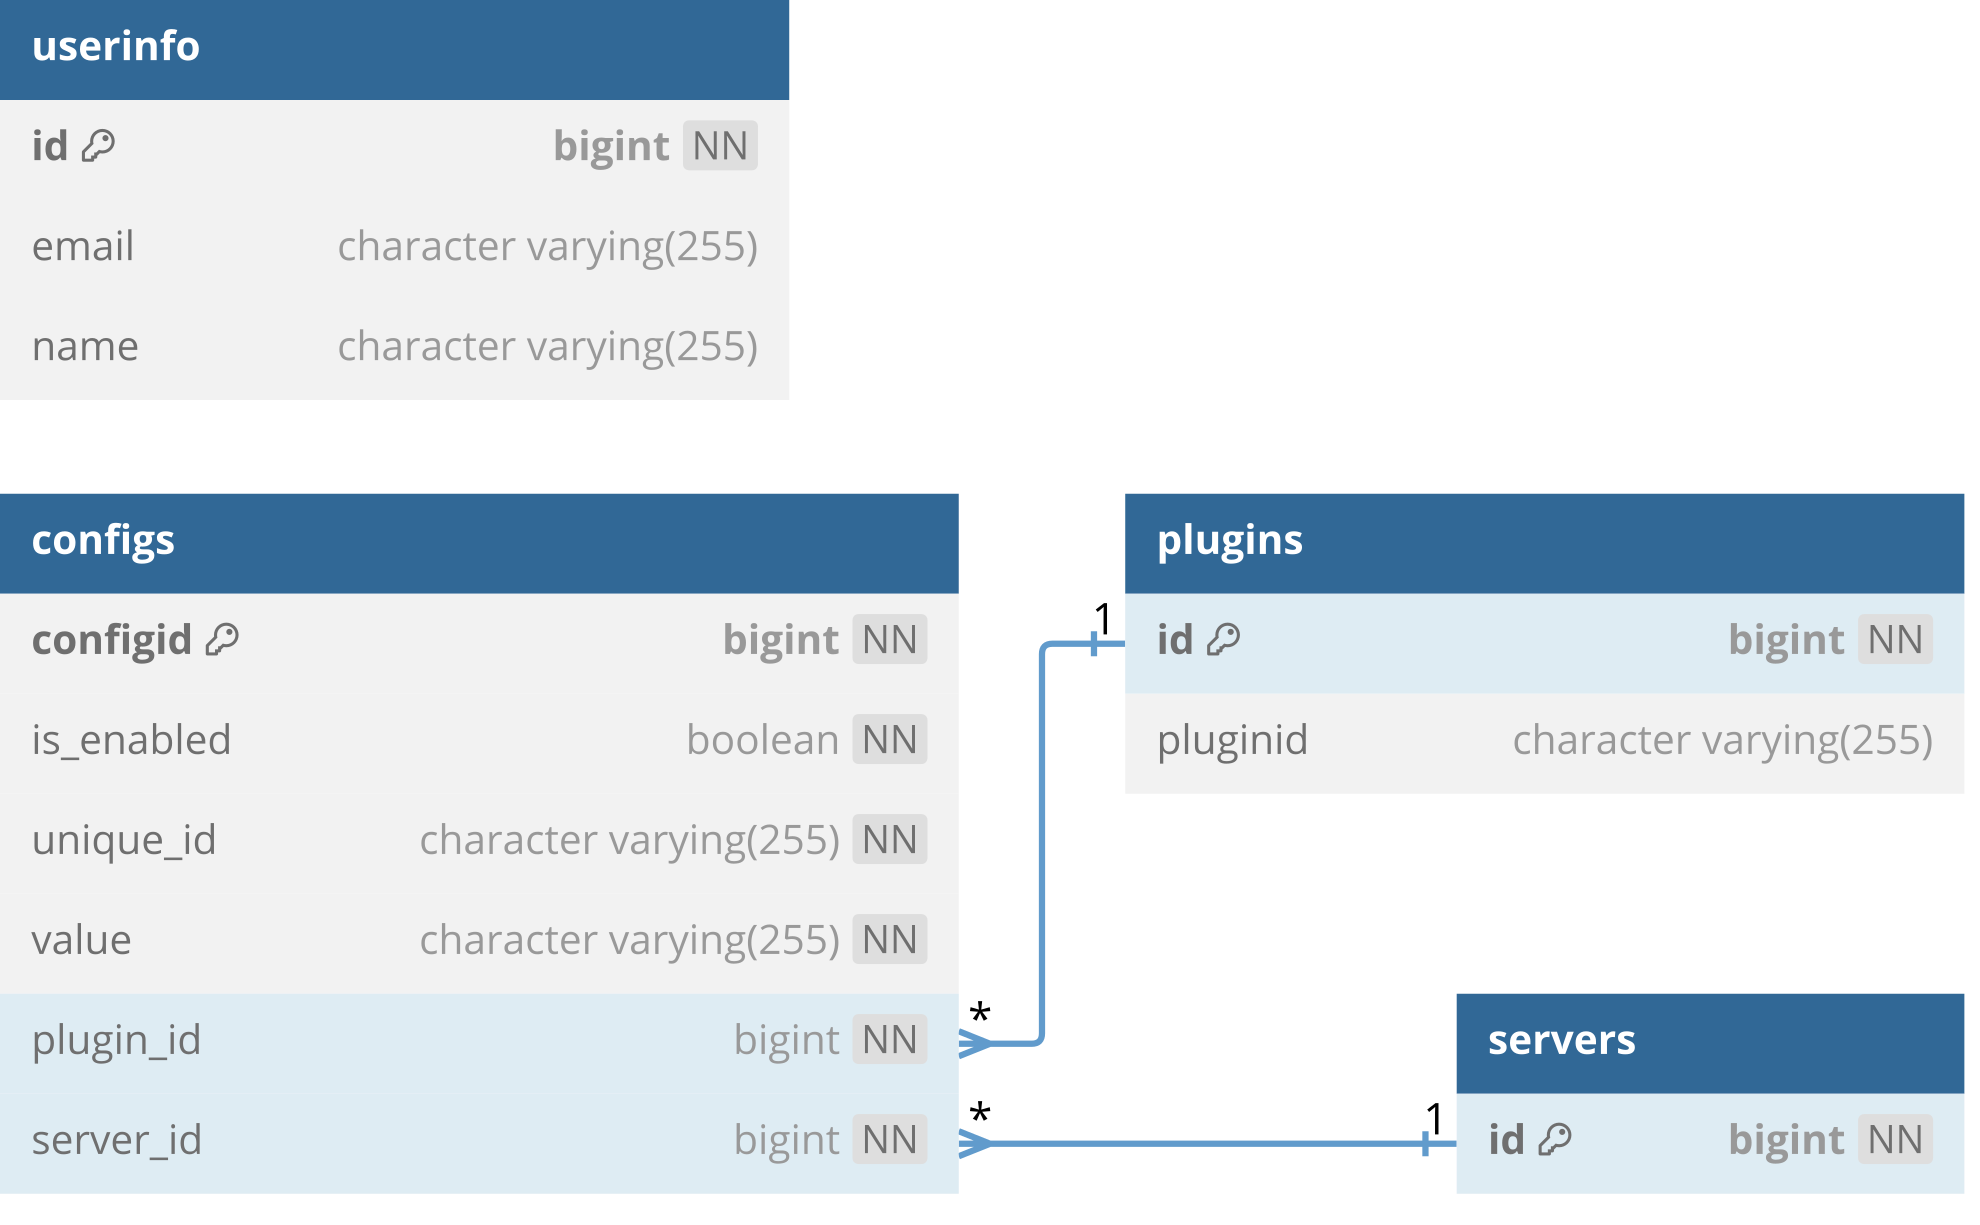
\includegraphics[width=\textwidth]{images/20240529-dbschema.png}
  \caption{Datenbankmodell}\label{fig:database-schema}
\end{figure}
  
\paragraph{\texorpdfstring{Tabelle \texttt{userinfo}}{Tabelle userinfo}}\label{tabelle-userinfo}
\begin{figure}[!htbp]
  \centering
  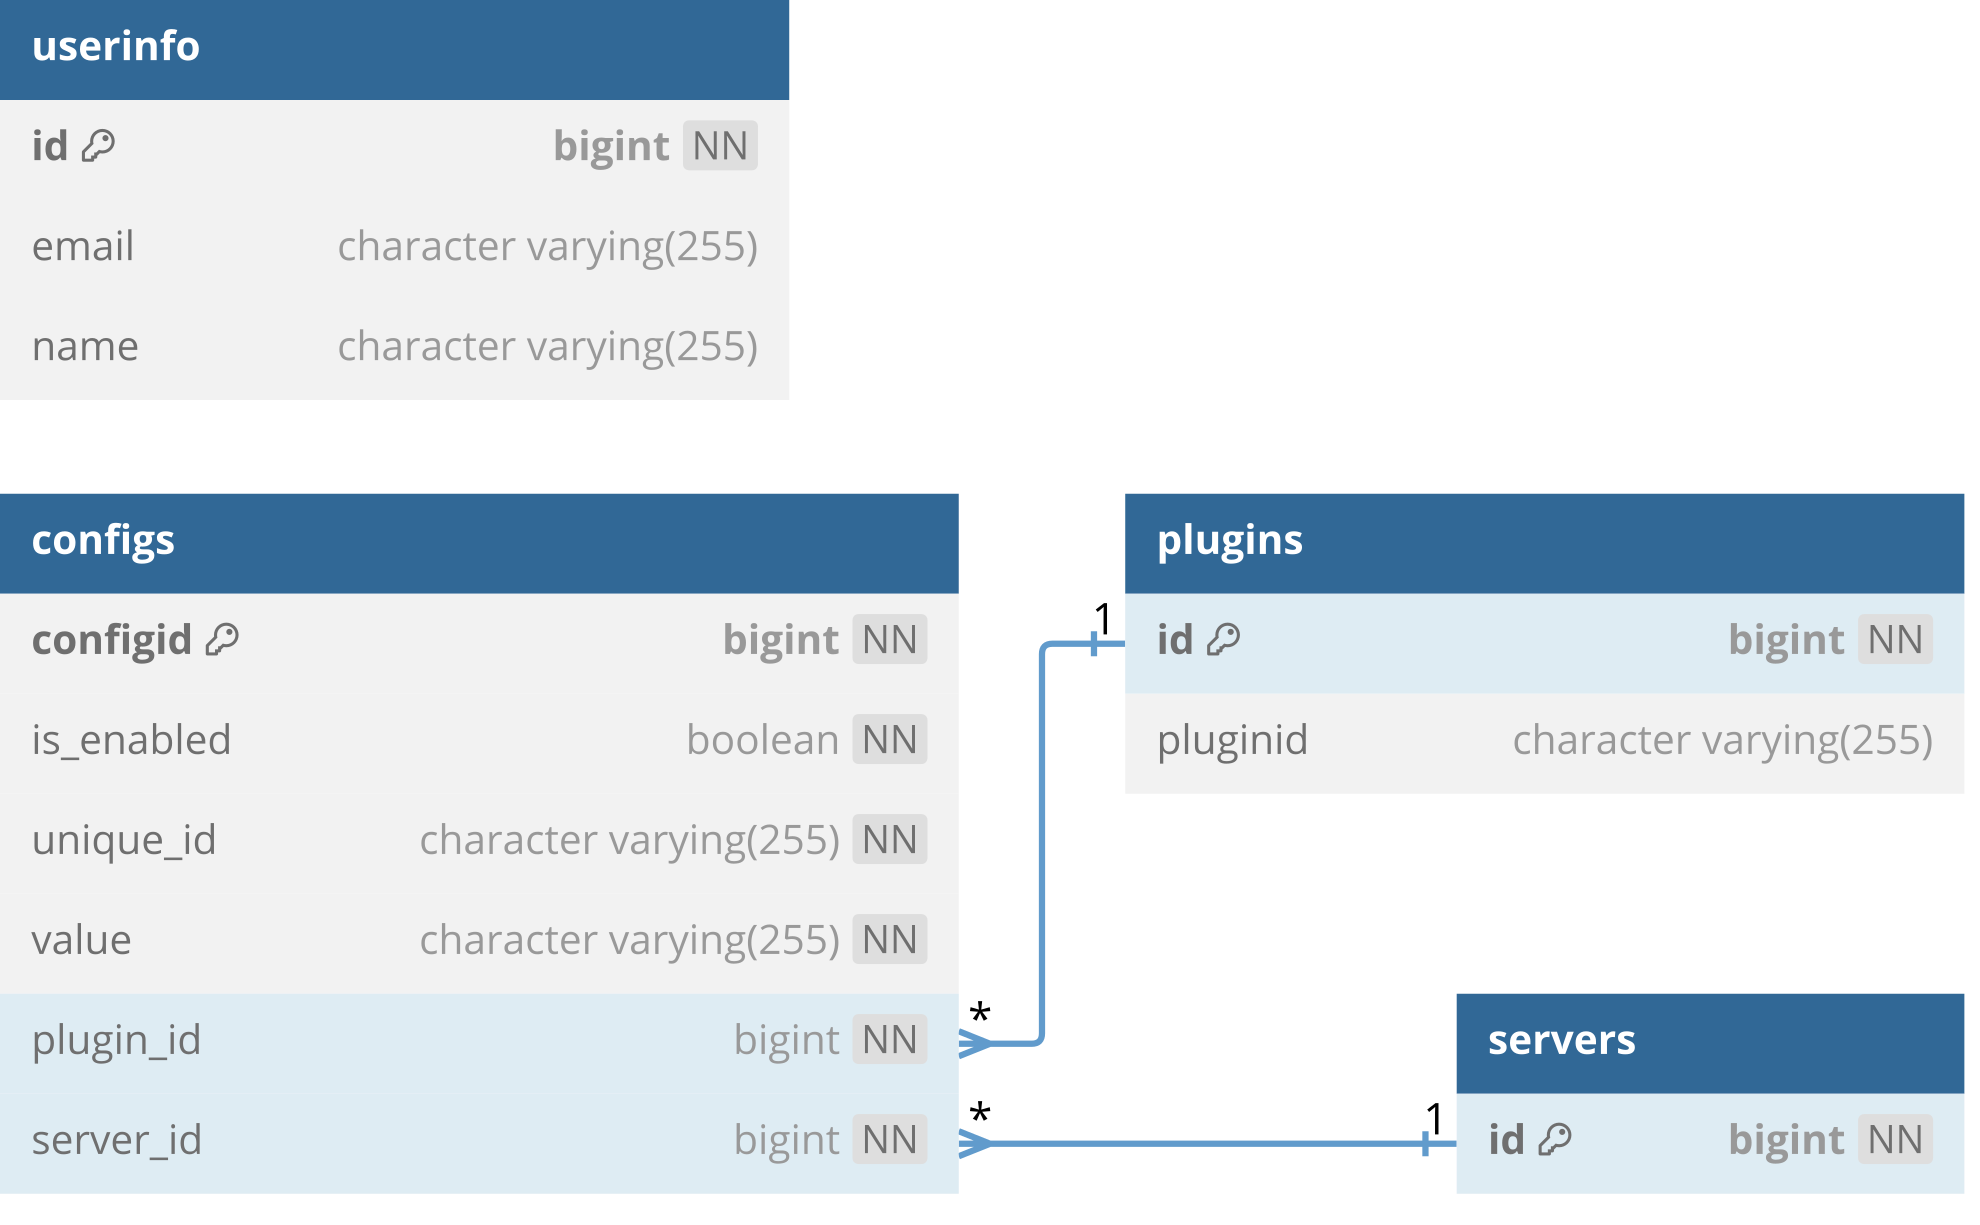
\includegraphics[width=\textwidth]{images/20240529-dbschema.png}
  \caption{Datenbankmodell}\label{fig:database-schema}
\end{figure}
  
\paragraph{\texorpdfstring{Tabelle \texttt{userinfo}}{Tabelle userinfo}}\label{tabelle-userinfo}

Die Tabelle \texttt{userinfo} speichert Informationen über die Benutzer der Anwendung. Jede Zeile repräsentiert einen einzelnen Benutzer.
Die Tabelle \texttt{userinfo} speichert Informationen über die Benutzer der Anwendung. Jede Zeile repräsentiert einen einzelnen Benutzer.

\begin{itemize}
\item
  \textbf{id} (BIGINT, PRIMARY KEY, NOT NULL): Eindeutige Identifikationsnummer des Benutzers. Dies ist der Primärschlüssel der Tabelle.
  \textbf{id} (BIGINT, PRIMARY KEY, NOT NULL): Eindeutige Identifikationsnummer des Benutzers. Dies ist der Primärschlüssel der Tabelle.
\item
  \textbf{email} (VARCHAR(255), NOT NULL): Die E-Mail-Adresse des Benutzers, die für Benachrichtigungen und Authentifizierungen verwendet wird.
  \textbf{email} (VARCHAR(255), NOT NULL): Die E-Mail-Adresse des Benutzers, die für Benachrichtigungen und Authentifizierungen verwendet wird.
\item
  \textbf{name} (VARCHAR(255), NOT NULL): Der Name des Benutzers, der zur Identifikation und Personalisierung der Benutzererfahrung verwendet wird.
  \textbf{name} (VARCHAR(255), NOT NULL): Der Name des Benutzers, der zur Identifikation und Personalisierung der Benutzererfahrung verwendet wird.
\end{itemize}

\paragraph{\texorpdfstring{Tabelle \texttt{plugins}}{Tabelle plugins}}\label{tabelle-plugins}
\paragraph{\texorpdfstring{Tabelle \texttt{plugins}}{Tabelle plugins}}\label{tabelle-plugins}

Die Tabelle \texttt{plugins} enthält Informationen über die verschiedenen Plugins, die in der Anwendung verwendet werden können. Jedes Plugin stellt eine eigenständige Erweiterung der Funktionalität dar.
Die Tabelle \texttt{plugins} enthält Informationen über die verschiedenen Plugins, die in der Anwendung verwendet werden können. Jedes Plugin stellt eine eigenständige Erweiterung der Funktionalität dar.

\begin{itemize}
\item
  \textbf{id} (BIGINT, PRIMARY KEY, NOT NULL): Eindeutige Identifikationsnummer des Plugins. Dies ist der Primärschlüssel der Tabelle.
  \textbf{id} (BIGINT, PRIMARY KEY, NOT NULL): Eindeutige Identifikationsnummer des Plugins. Dies ist der Primärschlüssel der Tabelle.
\item
  \textbf{pluginid} (VARCHAR(255), NOT NULL): Die Plugin-ID, die das Plugin eindeutig identifiziert. Diese ID wird verwendet, um das Plugin innerhalb der Anwendung zu referenzieren.
  \textbf{pluginid} (VARCHAR(255), NOT NULL): Die Plugin-ID, die das Plugin eindeutig identifiziert. Diese ID wird verwendet, um das Plugin innerhalb der Anwendung zu referenzieren.
\end{itemize}

\paragraph{\texorpdfstring{Tabelle \texttt{servers}}{Tabelle servers}}\label{tabelle-servers}
\paragraph{\texorpdfstring{Tabelle \texttt{servers}}{Tabelle servers}}\label{tabelle-servers}

Die Tabelle \texttt{servers} speichert Informationen über die Discord-Server, auf denen der Bot installiert ist. Diese Informationen sind wichtig, um die verschiedenen Instanzen des Bots auf den verschiedenen Servern zu verwalten.
Die Tabelle \texttt{servers} speichert Informationen über die Discord-Server, auf denen der Bot installiert ist. Diese Informationen sind wichtig, um die verschiedenen Instanzen des Bots auf den verschiedenen Servern zu verwalten.

\begin{itemize}
\item
  \textbf{id} (BIGINT, PRIMARY KEY, NOT NULL): Eindeutige Identifikationsnummer des Servers. Dies ist der Primärschlüssel der Tabelle.
  \textbf{id} (BIGINT, PRIMARY KEY, NOT NULL): Eindeutige Identifikationsnummer des Servers. Dies ist der Primärschlüssel der Tabelle.
\item
  \textbf{pluginid} (VARCHAR(255), NOT NULL): Die Plugin-ID, die dem Server zugeordnet ist. Diese ID hilft, die Plugins zu verwalten, die auf den einzelnen Servern installiert sind.
  \textbf{pluginid} (VARCHAR(255), NOT NULL): Die Plugin-ID, die dem Server zugeordnet ist. Diese ID hilft, die Plugins zu verwalten, die auf den einzelnen Servern installiert sind.
\end{itemize}

\paragraph{\texorpdfstring{Tabelle \texttt{configs}}{Tabelle configs}}\label{tabelle-configs}
\paragraph{\texorpdfstring{Tabelle \texttt{configs}}{Tabelle configs}}\label{tabelle-configs}

Die Tabelle \texttt{configs} speichert spezifische Konfigurationen für jedes Plugin auf einem Server. Diese Konfigurationen ermöglichen es, die Funktionsweise der Plugins auf den jeweiligen Servern anzupassen.
Die Tabelle \texttt{configs} speichert spezifische Konfigurationen für jedes Plugin auf einem Server. Diese Konfigurationen ermöglichen es, die Funktionsweise der Plugins auf den jeweiligen Servern anzupassen.

\begin{itemize}
\item
  \textbf{configid} (BIGINT, PRIMARY KEY, NOT NULL): Eindeutige Identifikationsnummer der Konfiguration. Dies ist der Primärschlüssel der Tabelle.
  \textbf{configid} (BIGINT, PRIMARY KEY, NOT NULL): Eindeutige Identifikationsnummer der Konfiguration. Dies ist der Primärschlüssel der Tabelle.
\item
  \textbf{is\_enabled} (BOOLEAN, NOT NULL): Ein Flag, das angibt, ob die Konfiguration aktiviert (TRUE) oder deaktiviert (FALSE) ist. Dies ermöglicht das einfache Ein- und Ausschalten von Plugin-Funktionen.
  \textbf{is\_enabled} (BOOLEAN, NOT NULL): Ein Flag, das angibt, ob die Konfiguration aktiviert (TRUE) oder deaktiviert (FALSE) ist. Dies ermöglicht das einfache Ein- und Ausschalten von Plugin-Funktionen.
\item
  \textbf{unique\_id} (VARCHAR(255), NOT NULL): Eine eindeutige ID, die zur Identifikation der Konfiguration dient. Diese ID wird verwendet, um spezifische Konfigurationseinstellungen zu referenzieren.
  \textbf{unique\_id} (VARCHAR(255), NOT NULL): Eine eindeutige ID, die zur Identifikation der Konfiguration dient. Diese ID wird verwendet, um spezifische Konfigurationseinstellungen zu referenzieren.
\item
  \textbf{value} (VARCHAR(255), NOT NULL): Der Wert der Konfiguration. Dies könnte z.B. eine bestimmte Einstellung oder ein Parameter sein, der die Funktionsweise des Plugins beeinflusst.
  \textbf{value} (VARCHAR(255), NOT NULL): Der Wert der Konfiguration. Dies könnte z.B. eine bestimmte Einstellung oder ein Parameter sein, der die Funktionsweise des Plugins beeinflusst.
\item
  \textbf{plugin\_id} (BIGINT, NOT NULL): Die ID des Plugins, zu dem diese Konfiguration gehört. Diese Spalte verweist auf \texttt{plugins.id} und ermöglicht es, die Konfigurationen spezifischen Plugins zuzuordnen.
  \textbf{plugin\_id} (BIGINT, NOT NULL): Die ID des Plugins, zu dem diese Konfiguration gehört. Diese Spalte verweist auf \texttt{plugins.id} und ermöglicht es, die Konfigurationen spezifischen Plugins zuzuordnen.
\item
  \textbf{server\_id} (BIGINT, NOT NULL): Die ID des Servers, auf dem das Plugin installiert ist. Diese Spalte verweist auf \texttt{servers.id} und hilft, die Konfigurationen den entsprechenden Servern zuzuordnen.
  \textbf{server\_id} (BIGINT, NOT NULL): Die ID des Servers, auf dem das Plugin installiert ist. Diese Spalte verweist auf \texttt{servers.id} und hilft, die Konfigurationen den entsprechenden Servern zuzuordnen.
\end{itemize}

\subsubsection{Beziehungen zwischen den Tabellen}\label{beziehungen-zwischen-den-tabellen}
\subsubsection{Beziehungen zwischen den Tabellen}\label{beziehungen-zwischen-den-tabellen}

Die Tabellen sind durch verschiedene Beziehungen miteinander verknüpft, um die Datenintegrität zu gewährleisten und die Struktur der Anwendung abzubilden.
Die Tabellen sind durch verschiedene Beziehungen miteinander verknüpft, um die Datenintegrität zu gewährleisten und die Struktur der Anwendung abzubilden.

\begin{itemize}
\item
  \textbf{Server und Plugins}: Ein Server (\texttt{servers}) kann mehrere Plugins (\texttt{plugins}) verwenden. Diese Beziehung wird durch die Verknüpfungstabelle \texttt{configs} realisiert. Die Tabelle \texttt{configs} enthält die Fremdschlüssel \texttt{configs.server\_id} und \texttt{configs.plugin\_id}, die auf \texttt{servers.id} bzw. \texttt{plugins.id} verweisen. Diese Tabelle ermöglicht es, die Konfiguration jedes Plugins für jeden Server individuell zu speichern.
  \textbf{Server und Plugins}: Ein Server (\texttt{servers}) kann mehrere Plugins (\texttt{plugins}) verwenden. Diese Beziehung wird durch die Verknüpfungstabelle \texttt{configs} realisiert. Die Tabelle \texttt{configs} enthält die Fremdschlüssel \texttt{configs.server\_id} und \texttt{configs.plugin\_id}, die auf \texttt{servers.id} bzw. \texttt{plugins.id} verweisen. Diese Tabelle ermöglicht es, die Konfiguration jedes Plugins für jeden Server individuell zu speichern.
\end{itemize}

\subsubsection{Detaillierte Beschreibung der Beziehungen}\label{detaillierte-beschreibung-der-beziehungen}

\paragraph{Server und Plugins (1:n Beziehung)}\label{server-und-plugins-1n-beziehung}
\subsubsection{Detaillierte Beschreibung der Beziehungen}\label{detaillierte-beschreibung-der-beziehungen}

\paragraph{Server und Plugins (1:n Beziehung)}\label{server-und-plugins-1n-beziehung}

\begin{itemize}
\item
  \textbf{Primärschlüssel}: \texttt{servers.id}, \texttt{plugins.id}
\item
  \textbf{Fremdschlüssel}: \texttt{configs.server\_id}, \texttt{configs.plugin\_id}
  \textbf{Fremdschlüssel}: \texttt{configs.server\_id}, \texttt{configs.plugin\_id}
\item
  \textbf{Beschreibung}: Ein Server kann mehrere Plugins verwenden, und ein Plugin kann auf mehreren Servern verwendet werden. Diese 1:n-Beziehung wird durch die \texttt{configs}-Tabelle vermittelt, die die IDs der Server und Plugins sowie die Konfigurationseinstellungen für die Plugins auf den jeweiligen Servern speichert.
  \textbf{Beschreibung}: Ein Server kann mehrere Plugins verwenden, und ein Plugin kann auf mehreren Servern verwendet werden. Diese 1:n-Beziehung wird durch die \texttt{configs}-Tabelle vermittelt, die die IDs der Server und Plugins sowie die Konfigurationseinstellungen für die Plugins auf den jeweiligen Servern speichert.
\end{itemize}

Die Datenbankstruktur und das Modell bieten die Grundlage für die Verwaltung von Benutzern, Discord-Servern und Plugins. Die klar definierten Beziehungen zwischen den Tabellen gewährleisten eine hohe Datenintegrität und ermöglichen eine flexible und erweiterbare Architektur für die Anwendung. Die Tabelle \texttt{userinfo} speichert Benutzerinformationen, die Tabelle \texttt{servers} speichert Serverinformationen, die Tabelle \texttt{plugins} speichert Plugin-Informationen, und die Tabelle \texttt{configs} speichert die Zuordnungen und Konfigurationen der Plugins zu den jeweiligen Servern.

Die Datenbankstruktur und das Modell bieten die Grundlage für die Verwaltung von Benutzern, Discord-Servern und Plugins. Die klar definierten Beziehungen zwischen den Tabellen gewährleisten eine hohe Datenintegrität und ermöglichen eine flexible und erweiterbare Architektur für die Anwendung. Die Tabelle \texttt{userinfo} speichert Benutzerinformationen, die Tabelle \texttt{servers} speichert Serverinformationen, die Tabelle \texttt{plugins} speichert Plugin-Informationen, und die Tabelle \texttt{configs} speichert die Zuordnungen und Konfigurationen der Plugins zu den jeweiligen Servern.


\subsubsection{Design Patterns}\label{design-patterns}

Während der Entwicklung wurden mehrere \gls{Design Patterns} eingesetzt, um die Codequalität und Wartbarkeit zu verbessern. Die folgenden Design Patterns wurden verwendet:

\paragraph{Singleton}\label{singleton} Ein Singleton-Entwurfsmuster wurde verwendet, um sicherzustellen, dass nur eine Instanz einer Klasse erstellt wird und auf diese Instanz global zugegriffen werden kann. Dies wurde für Klassen wie die Konfigurationsverwaltung verwendet, um sicherzustellen, dass nur eine Instanz der Konfiguration existiert und von verschiedenen Teilen der Anwendung verwendet werden kann. Bei einem Singleton-Designmuster wird eine statische Instanz der Klasse erstellt und auf diese Instanz über eine statische Methode zugegriffen. In Java kann dies durch die Verwendung des Schlüsselworts \texttt{static} und einer privaten Konstruktor-Methode erreicht werden:

\begin{lstlisting}[
  ,language=Java
  ,caption={Singleton-Entwurfsmuster in Java}
  ,label={lst:singleton}
]
public class Configuration {
    private static Configuration instance = null;
    private Configuration() {
        // private constructor to prevent instantiation
    }
    public static Configuration getInstance() {
        if (instance == null) {
            instance = new Configuration();
        }
        return instance;
    }
}
\end{lstlisting}

\paragraph{Factory}\label{factory} Ein Factory-Entwurfsmuster wurde verwendet, um die Erstellung von Objekten zu kapseln und die Flexibilität und Wiederverwendbarkeit des Codes zu erhöhen. Dies wurde für die Erstellung von Server- und Plugin-Objekten verwendet, um die Komplexität der Erstellung und Konfiguration dieser Objekte zu reduzieren. Bei einem Factory-Entwurfsmuster wird eine separate Fabrikmethode verwendet, um Objekte zu erstellen und zu konfigurieren. Dies ermöglicht es, die Erstellung von Objekten zu kapseln und die Implementierungsdetails zu verbergen. In Java kann dies durch die Verwendung einer statischen Fabrikmethode erreicht werden:

\begin{lstlisting}[
  ,language=Java
  ,caption={Factory-Entwurfsmuster in Java}
  ,label={lst:factory}
]
public class ServerFactory {
    public static Server createServer(String name, User owner) {
        Server server = new Server();
        server.setName(name);
        server.setOwner(owner);
        return server;
    }
}
\end{lstlisting}

\paragraph{Observer}\label{observer} Ein Observer-Entwurfsmuster wurde verwendet, um eine lose Kopplung zwischen Objekten zu ermöglichen und Event-Handling-Mechanismen zu implementieren. Dies wurde für die Implementierung von Benachrichtigungen und Ereignissen in der Anwendung verwendet. Bei einem Observer-Entwurfsmuster werden Beobachter- und Subjektobjekte verwendet, um Änderungen in einem Objekt zu überwachen und darauf zu reagieren. Dies ermöglicht es, Änderungen in einem Objekt zu verfolgen und andere Teile der Anwendung darüber zu informieren. In Java kann dies durch die Verwendung von Observer- und Observable-Klassen erreicht werden:


\begin{lstlisting}[
  ,language=Java
  ,caption={Observer-Entwurfsmuster in Java}
  ,label={lst:observer}
]
public class Subject extends Observable {
    public void notifyObservers(Object arg) {
        setChanged();
        super.notifyObservers(arg);
    }
}
public class Observer implements java.util.Observer {
    public void update(Observable o, Object arg) {
        // handle update
    }
}
\end{lstlisting}

Diese Design Patterns wurden ausgewählt, weil sie bewährte Lösungen für häufig auftretende Probleme bieten und die Codebasis strukturierter und erweiterbarer machen.
Während der Entwicklung wurden mehrere \gls{Design Patterns} eingesetzt, um die Codequalität und Wartbarkeit zu verbessern. Die folgenden Design Patterns wurden verwendet:

\paragraph{Singleton}\label{singleton} Ein Singleton-Entwurfsmuster wurde verwendet, um sicherzustellen, dass nur eine Instanz einer Klasse erstellt wird und auf diese Instanz global zugegriffen werden kann. Dies wurde für Klassen wie die Konfigurationsverwaltung verwendet, um sicherzustellen, dass nur eine Instanz der Konfiguration existiert und von verschiedenen Teilen der Anwendung verwendet werden kann. Bei einem Singleton-Designmuster wird eine statische Instanz der Klasse erstellt und auf diese Instanz über eine statische Methode zugegriffen. In Java kann dies durch die Verwendung des Schlüsselworts \texttt{static} und einer privaten Konstruktor-Methode erreicht werden:

\begin{lstlisting}[
  ,language=Java
  ,caption={Singleton-Entwurfsmuster in Java}
  ,label={lst:singleton}
]
public class Configuration {
    private static Configuration instance = null;
    private Configuration() {
        // private constructor to prevent instantiation
    }
    public static Configuration getInstance() {
        if (instance == null) {
            instance = new Configuration();
        }
        return instance;
    }
}
\end{lstlisting}

\paragraph{Factory}\label{factory} Ein Factory-Entwurfsmuster wurde verwendet, um die Erstellung von Objekten zu kapseln und die Flexibilität und Wiederverwendbarkeit des Codes zu erhöhen. Dies wurde für die Erstellung von Server- und Plugin-Objekten verwendet, um die Komplexität der Erstellung und Konfiguration dieser Objekte zu reduzieren. Bei einem Factory-Entwurfsmuster wird eine separate Fabrikmethode verwendet, um Objekte zu erstellen und zu konfigurieren. Dies ermöglicht es, die Erstellung von Objekten zu kapseln und die Implementierungsdetails zu verbergen. In Java kann dies durch die Verwendung einer statischen Fabrikmethode erreicht werden:

\begin{lstlisting}[
  ,language=Java
  ,caption={Factory-Entwurfsmuster in Java}
  ,label={lst:factory}
]
public class ServerFactory {
    public static Server createServer(String name, User owner) {
        Server server = new Server();
        server.setName(name);
        server.setOwner(owner);
        return server;
    }
}
\end{lstlisting}

\paragraph{Observer}\label{observer} Ein Observer-Entwurfsmuster wurde verwendet, um eine lose Kopplung zwischen Objekten zu ermöglichen und Event-Handling-Mechanismen zu implementieren. Dies wurde für die Implementierung von Benachrichtigungen und Ereignissen in der Anwendung verwendet. Bei einem Observer-Entwurfsmuster werden Beobachter- und Subjektobjekte verwendet, um Änderungen in einem Objekt zu überwachen und darauf zu reagieren. Dies ermöglicht es, Änderungen in einem Objekt zu verfolgen und andere Teile der Anwendung darüber zu informieren. In Java kann dies durch die Verwendung von Observer- und Observable-Klassen erreicht werden:


\begin{lstlisting}[
  ,language=Java
  ,caption={Observer-Entwurfsmuster in Java}
  ,label={lst:observer}
]
public class Subject extends Observable {
    public void notifyObservers(Object arg) {
        setChanged();
        super.notifyObservers(arg);
    }
}
public class Observer implements java.util.Observer {
    public void update(Observable o, Object arg) {
        // handle update
    }
}
\end{lstlisting}

Diese Design Patterns wurden ausgewählt, weil sie bewährte Lösungen für häufig auftretende Probleme bieten und die Codebasis strukturierter und erweiterbarer machen.

\subsection{Qualitätssicherung}\label{qualituxe4tssicherung}

\subsubsection{Code Reviews}\label{code-reviews}

Während der Entwicklung wurden regelmäßige Code-Reviews durchgeführt, um sicherzustellen, dass der Code qualitativ hochwertig und fehlerfrei ist. Die Code-Reviews wurden von den Teammitgliedern durchgeführt, die nicht an der ursprünglichen Implementierung beteiligt waren. Dies ermöglichte es, potenzielle Fehler und Probleme frühzeitig zu identifizieren und zu beheben. Die Code-Reviews konzentrierten sich auf Aspekte wie Code-Qualität, Lesbarkeit, Wartbarkeit, Performance und Sicherheit. Die Ergebnisse der Code-Reviews wurden dokumentiert und in die weitere Entwicklung integriert.

\subsubsection{Code Reviews}\label{code-reviews}

Während der Entwicklung wurden regelmäßige Code-Reviews durchgeführt, um sicherzustellen, dass der Code qualitativ hochwertig und fehlerfrei ist. Die Code-Reviews wurden von den Teammitgliedern durchgeführt, die nicht an der ursprünglichen Implementierung beteiligt waren. Dies ermöglichte es, potenzielle Fehler und Probleme frühzeitig zu identifizieren und zu beheben. Die Code-Reviews konzentrierten sich auf Aspekte wie Code-Qualität, Lesbarkeit, Wartbarkeit, Performance und Sicherheit. Die Ergebnisse der Code-Reviews wurden dokumentiert und in die weitere Entwicklung integriert.

\subsubsection{Teststrategien}\label{teststrategien}

Für die Qualitätssicherung wurden verschiedene Teststrategien eingesetzt, um sicherzustellen, dass die Anwendung stabil und fehlerfrei funktioniert.

Für die Qualitätssicherung wurden verschiedene Teststrategien eingesetzt, um sicherzustellen, dass die Anwendung stabil und fehlerfrei funktioniert.

\begin{itemize}
  \item
        **Unit Tests**: Diese Tests wurden auf der kleinsten Code-Ebene durchgeführt, um sicherzustellen, dass einzelne Methoden und Funktionen korrekt arbeiten. Dabei kamen JUnit und Mockito zum Einsatz.
  \item
        **Integrationstests**: Diese Tests überprüften das Zusammenspiel mehrerer Komponenten und Dienste der Anwendung. Hierbei wurde insbesondere die Integration der Datenbank und der REST-API getestet.
        **Unit Tests**: Diese Tests wurden auf der kleinsten Code-Ebene durchgeführt, um sicherzustellen, dass einzelne Methoden und Funktionen korrekt arbeiten. Dabei kamen JUnit und Mockito zum Einsatz.
  \item
        **Integrationstests**: Diese Tests überprüften das Zusammenspiel mehrerer Komponenten und Dienste der Anwendung. Hierbei wurde insbesondere die Integration der Datenbank und der REST-API getestet.
  \item
        **Systemtests**: Diese Tests wurden durchgeführt, um das gesamte System unter realistischen Bedingungen zu überprüfen. Dazu gehörten Tests der Benutzeroberfläche und der API-Endpunkte.
        **Systemtests**: Diese Tests wurden durchgeführt, um das gesamte System unter realistischen Bedingungen zu überprüfen. Dazu gehörten Tests der Benutzeroberfläche und der API-Endpunkte.
\end{itemize}

\subsubsection{Testfälle}\label{testfuxe4lle}

Konkrete Testfälle:

Konkrete Testfälle:

\begin{itemize}
  \item
        **Benutzerregistrierung**: Testfall zur Überprüfung der erfolgreichen Registrierung eines neuen Benutzers. Erwartetes Ergebnis: Der Benutzer wird in der Datenbank gespeichert und kann sich anmelden.
  \item
        **Plugin-Aktivierung**: Testfall zur Überprüfung der erfolgreichen Aktivierung eines Plugins auf einem Server. Erwartetes Ergebnis: Das Plugin wird aktiviert und die entsprechende Konfiguration wird gespeichert.
  \item
        **Server-Verwaltung**: Testfall zur Überprüfung der korrekten Erstellung und Verwaltung von Servern. Erwartetes Ergebnis: Server werden korrekt in der Datenbank gespeichert und können vom Benutzer verwaltet werden.
        **Benutzerregistrierung**: Testfall zur Überprüfung der erfolgreichen Registrierung eines neuen Benutzers. Erwartetes Ergebnis: Der Benutzer wird in der Datenbank gespeichert und kann sich anmelden.
  \item
        **Plugin-Aktivierung**: Testfall zur Überprüfung der erfolgreichen Aktivierung eines Plugins auf einem Server. Erwartetes Ergebnis: Das Plugin wird aktiviert und die entsprechende Konfiguration wird gespeichert.
  \item
        **Server-Verwaltung**: Testfall zur Überprüfung der korrekten Erstellung und Verwaltung von Servern. Erwartetes Ergebnis: Server werden korrekt in der Datenbank gespeichert und können vom Benutzer verwaltet werden.
\end{itemize}

\subsubsection{Zusammenfassung der Testergebnisse}

Die durchgeführten Tests haben gezeigt, dass die Anwendung stabil und funktional ist. Alle kritischen Funktionen wurden erfolgreich getestet und funktionieren wie erwartet. Es wurden keine schwerwiegenden Fehler gefunden, und kleinere Bugs wurden behoben. Die Anwendung erfüllt die gestellten Anforderungen und ist bereit für den Einsatz.
